%%%%%%%%%%%%%%%%%%%%%%%%%%%%%%%%%%%%%%%%%%%%%%%%%%%%%%%%%%%%%%%%%%%%%%%%%%%%%%%%
% experiment.tex: Chapter describing the experiment
%%%%%%%%%%%%%%%%%%%%%%%%%%%%%%%%%%%%%%%%%%%%%%%%%%%%%%%%%%%%%%%%%%%%%%%%%%%%%%%%
\chapter{The Large Hadron Collider and CMS Experiment}
\label{sec:experiment_chapter}
%%%%%%%%%%%%%%%%%%%%%%%%%%%%%%%%%%%%%%%%%%%%%%%%%%%%%%%%%%%%%%%%%%%%%%%%%%%%%%%%
%\subsection{Overview of the Compact Muon Solenoid and Large Hadron Collider}
The Compact Muon Solenoid (CMS) experiment was built to detect all Standard Model (SM) particles, and to
search for any interactions, predicted by the SM or not, that produced SM particles, like the extended 
weak interaction described in Chapter ~\ref{wrBosonAndHeavyNu}.  The CERN Large Hadron Collider (LHC) 
collided high-energy protons at the geometric center of the CMS experiment, and the results of proton-proton (pp) 
interactions were recorded.

The results of pp interactions were recorded if any of the following were detected:
\begin{itemize}
	\item one or more energetic charged leptons (electron, muon, tau or their anti-particles)
	\item one or more energetic photons
	\item one or more energetic hadronic jets, each containing at least one hadron
	\item one or more energetic neutrinos\footnote{the presence of neutrinos is inferred by measuring a net imbalance in 
		momentum from all detected charged leptons, photons and jets in a collision event.}
	\item combinations thereof
\end{itemize}
Particles produced by pp interactions were detected using a 3.8$\unit{T}$ magnet and four CMS 
sub-detector systems.  The important aspects of each sub-detector system are presented here, and a more detailed 
description is given elsewhere \cite{cmsDetectorPaper}.  As shown in Figure \ref{fig:layersOfCMS}, the nominal pp interaction point 
was surrounded by the silicon tracker where charged particles were first detected.  As charged particles traversed
the tracker, mobile electron-hole (e-h) pairs were created along their trajectories.  The tracker detected 
charged particles by counting the number of e-h pairs created.

\begin{figure}[h]
	\centering
	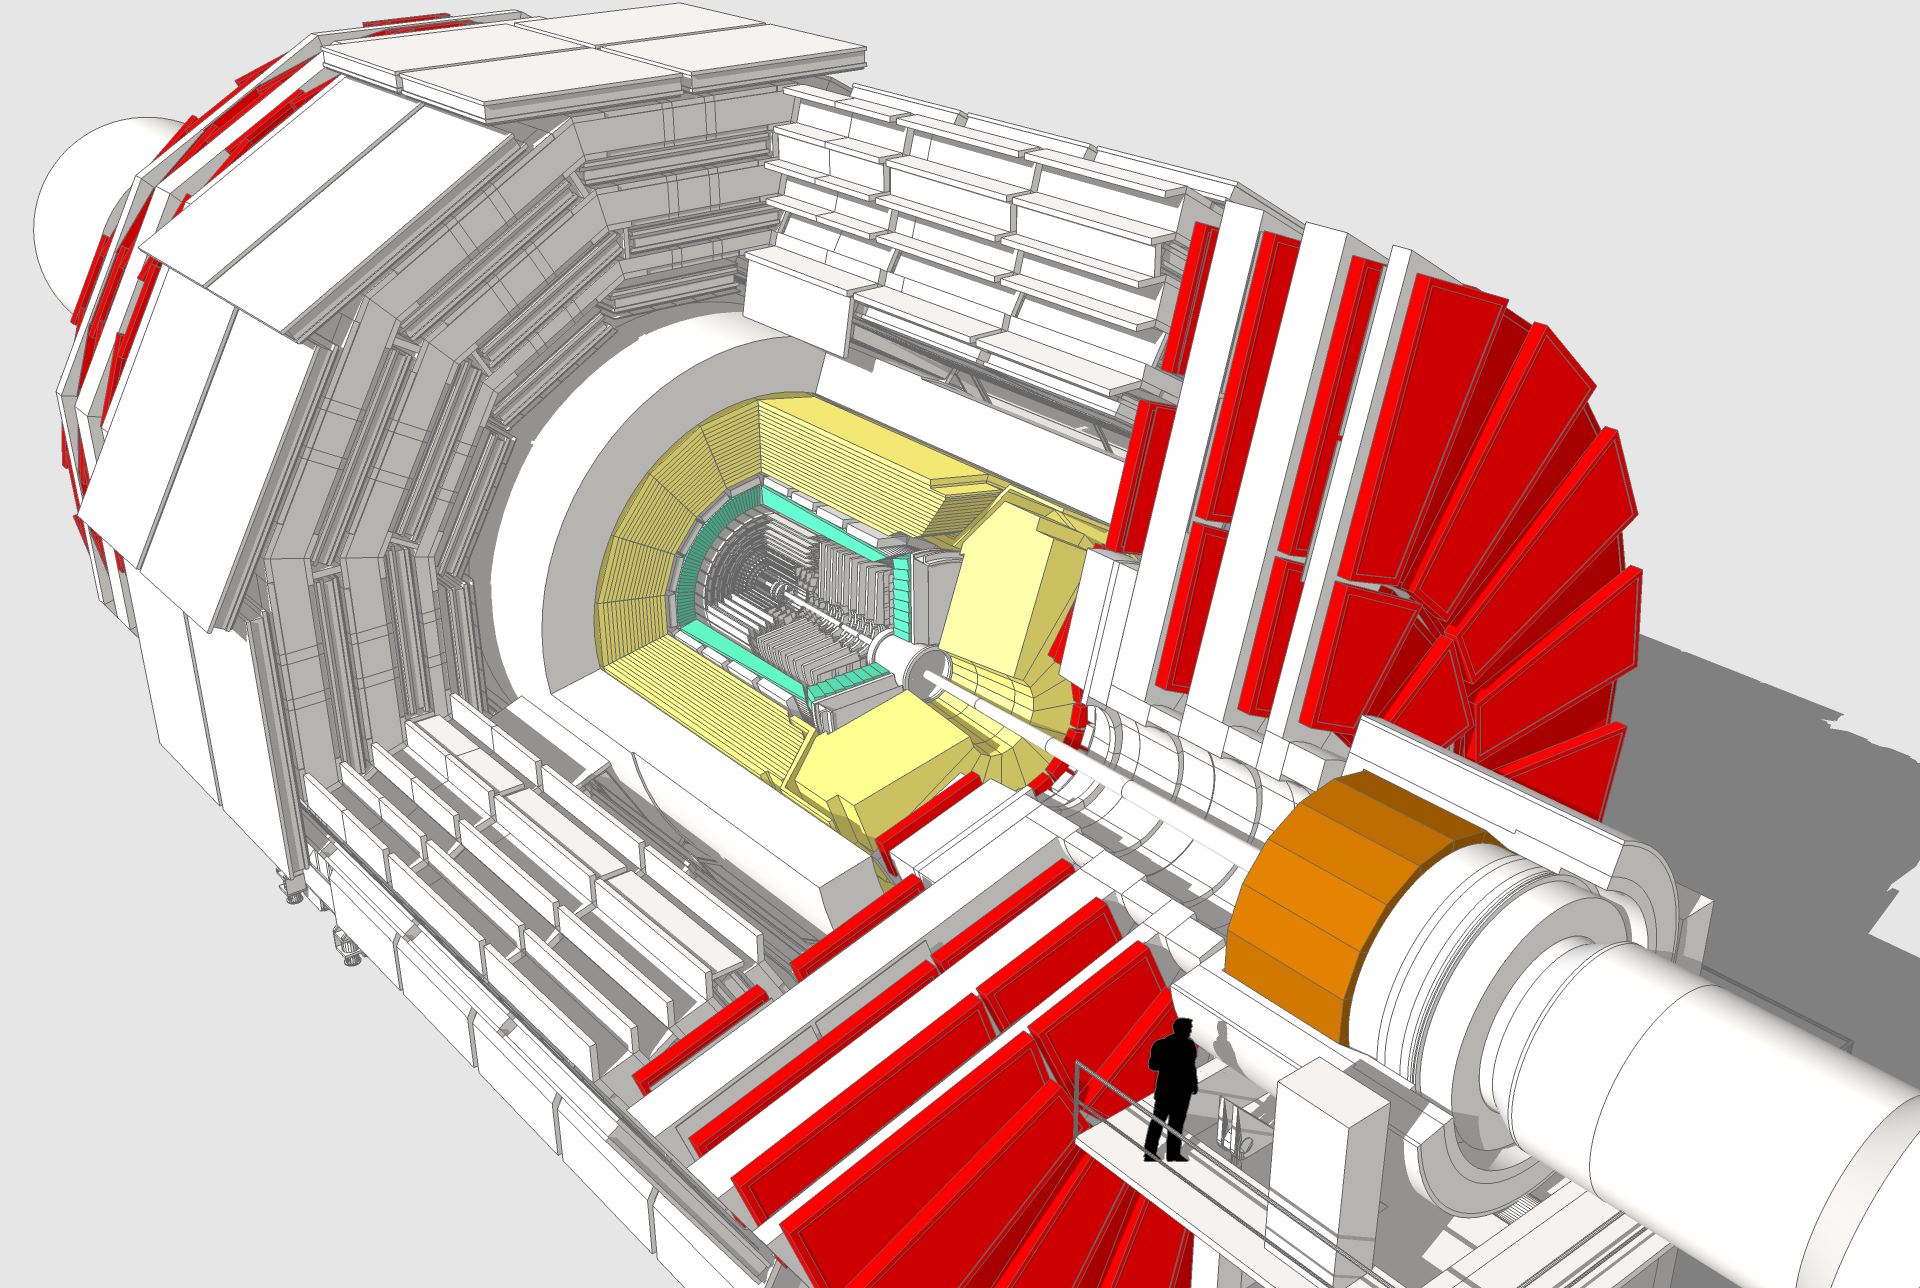
\includegraphics[width=1\textwidth]{figures/cmsDetectorBasic.png}
	\caption{Cut-away view of the entire CMS detector.  Closest to the proton-proton collision/interaction point is the 
		silicon tracker, followed by the Electromagnetic Calorimeter, then the Hadronic Calorimeter, and the 
	magnet.  Outside the magnet solenoid are the muon detectors.}
	\label{fig:layersOfCMS}
\end{figure}


Surrounding the silicon tracker was the lead-tungstate crystal (PbWO$_{4}$) Electromagnetic Calorimeter (ECAL).  
The ECAL was an absorption calorimeter that detected photons, and distinguished electrons and positrons from other charged 
particles detected by the tracker.  Electrons, positrons and photons interacted with lead-tungstate nuclei, 
produced showers of lower energy $e^{\pm}$ that interacted with atomic electrons in PbWO$_{4}$, and subsequently 
emitted visible light through fast ($\lesssim$20 \ns) scintillation.  Electrons, positrons and photons produced 
by pp interactions were detected by measuring the visible light produced by PbWO$_{4}$ crystals.

Wrapped around the ECAL was the Hadronic Calorimeter (HCAL).  Built from alternating layers of brass absorber and 
scintillating plastic tiles, the HCAL was a sampling calorimeter that detected hadrons in jets.  Hadrons that 
reached the HCAL interacted with nucleons in brass absorber layers, produced showers of 
lower energy hadrons that interacted with plastic scintillator molecules, which then emitted visible light through 
fast ($\lesssim$10 \ns) scintillation.  Hadrons in jets produced by pp interactions were detected by measuring the 
visible light produced by scintillating plastic tiles.

Outside the HCAL was the solenoid magnet that generated a 3.8$\unit{T}$ field.  The magnetic field was generated by running a current of 
$\lesssim$18000 amps through superconducting wire wound into a solenoid.  The wire, made from a niobium alloy, was 
cooled to a superconducting state using a cryogenic system adjacent to the solenoid.  The magnet and its subsystems 
were supported by a structure made mostly from iron, through which only muons could penetrate.

Surrounding the magnet were the muon detectors, which resided 
in the magnet iron return yoke where the magnetic field strength was between 1 and 3$\unit{T}$.  Three 
different technologies - drift tubes (DT) in the lowest radiation regions, cathode strip chambers (CSC) in higher 
radiation regions, and resistive plate chambers (RPC) in all regions - were used to detect muons.  In all muon detectors 
muons travelled through pressurized gas chambers and ionized electrons from the gas along their 
trajectories.  Within the chambers, electric fields accelerated the ionized electrons towards conducting wires.  Muons 
were detected by measuring the charge collected by conducting wires.

Due to the enormous rate of pp collisions in which only elastic or diffractive scattering occurred between protons, a two tiered trigger 
system was used to select events where energetic charged leptons, hadronic jets, photons, neutrinos or combinations 
thereof were detected.  The first tier of the trigger system processed information from the ECAL, the HCAL and the muon 
detectors in small regions where high energy particles were detected.  High energy regions identified by the first tier 
were then processed by the second tier trigger system.  In the second tier, reconstruction software 
was run in high energy regions to identify charged leptons, photons, jets and neutrinos.  If a pp collision event resulted in 
one or more reconstructed particles that passed energy and quality selections defined in the second tier, then all data 
from all four sub-detector systems for that event was read out and written to permanent storage.

The accelerator that collided protons, the coordinate system used to characterize the kinematics of detected 
particles, the four sub-detector systems and the trigger system are discussed in this chapter.

\section{The Large Hadron Collider}
\label{sec:lhcDescription}
Situated near Geneva, Switzerland and spanning the French-Swiss border, the CERN Large Hadron Collider (LHC) accelerated 
two counter-rotating proton beams in a 27 km circular tunnel \cite{lhcTDR} to an energy of 6.5 TeV in 2015.  At several points along the tunnel 
the two beams collided, and surrounding one of these points the CMS experiment was built.

Several accelerator stages, shown in Figure \ref{fig:accelComplex} \cite{cernAccelSys}, were used to create each proton beam in the LHC.  
Each proton beam began as isolated proton bunches ionized from hydrogen gas.  Proton bunches were then accelerated to higher 
energies in 3 accelerator stages before they were injected into the LHC.  Once enough proton bunches were 
collected in the LHC (up to $\sim$2300 for each beam), the LHC created two proton beams with proton bunches separated by 
25\ns, and accelerated both beams to an energy of 6.5 TeV.

\begin{figure}[ht]
	\centering
	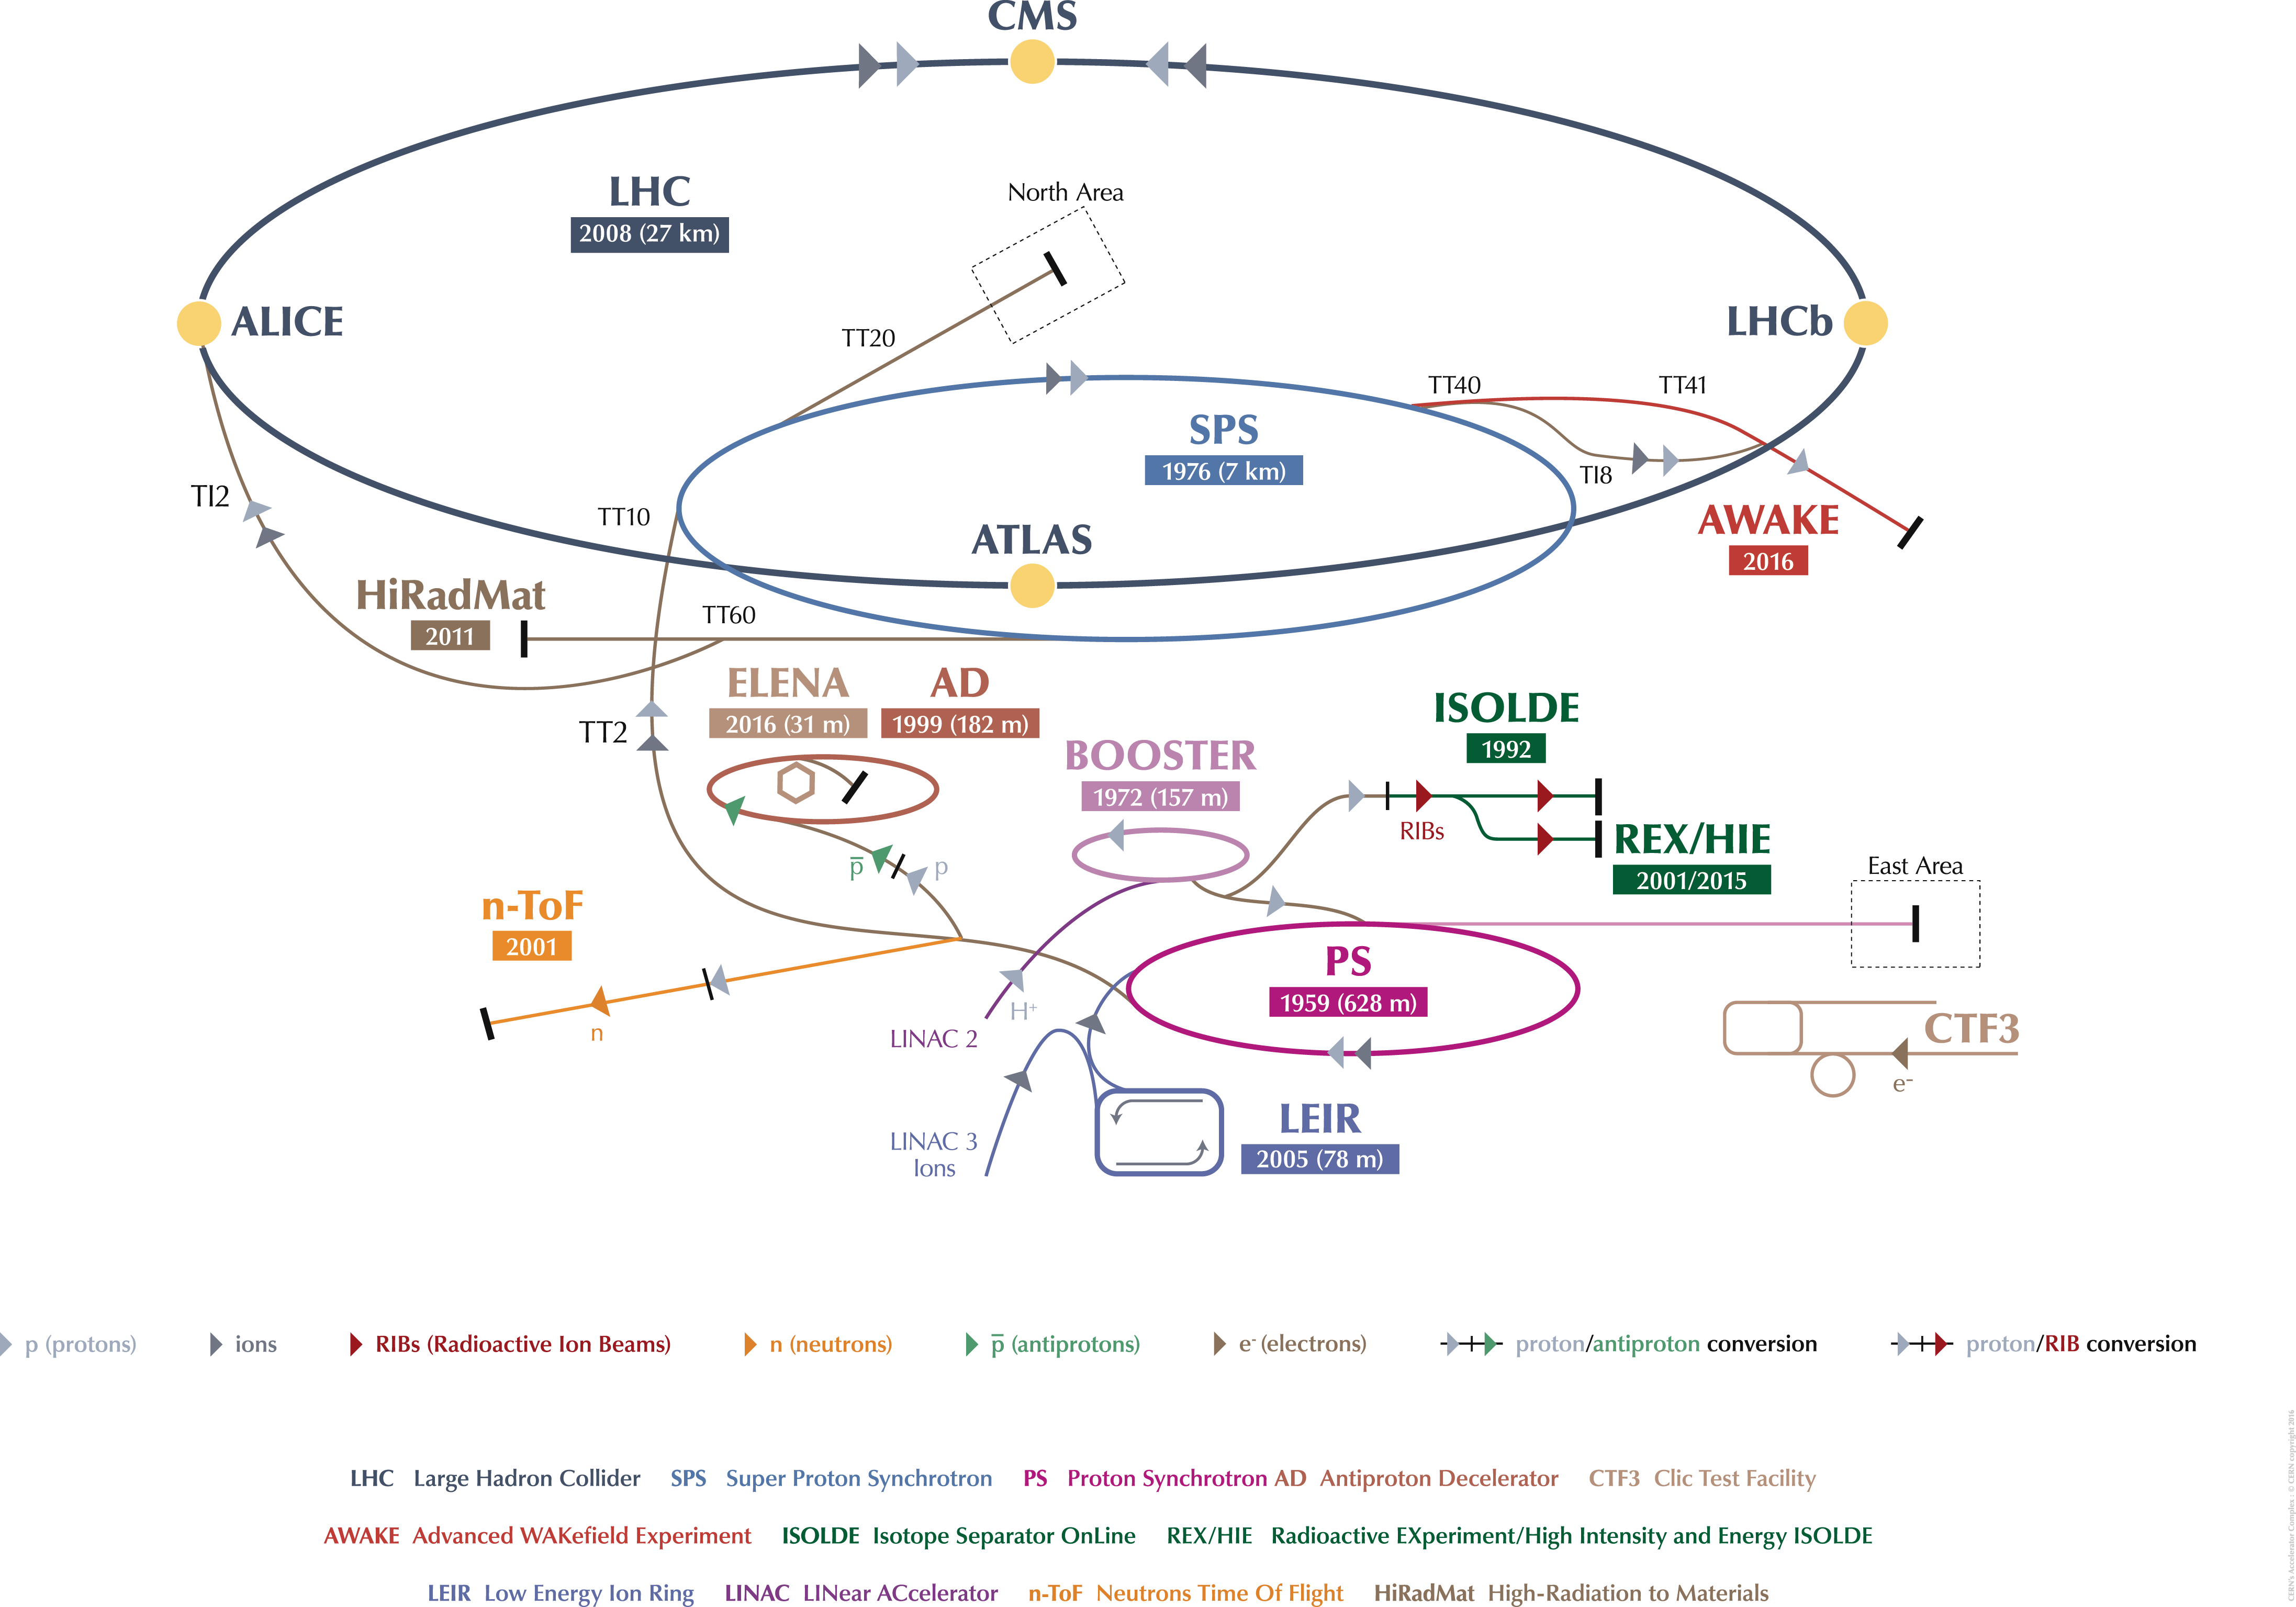
\includegraphics[width=1\textwidth]{figures/CERNAcceleratorComplex.png}
	\caption{The CERN accelerator complex.  Protons are ionized from hydrogen, then are accelerated to higher 
	energies by LINAC 2, the PS, and finally the SPS before entering the LHC.}
	\label{fig:accelComplex}
\end{figure}


In the LHC tunnel, superconducting radio-frequency (RF) cavities accelerated proton bunches, and magnets steered and 
focused the beams towards the collision point at the heart of CMS.  
During 2015 data taking the LHC collided protons at intensities approaching $6 \times 10^{33} \frac{1}{cm^{2}s}$ ($\sim 0.02 \frac{1}{fb\thickspace hr}$).  
From September through November 2015, CMS recorded 2.6 $fb^{-1}$ of collision events at $\sqrt{s} =$ 13 TeV.

\section{The CMS Coordinate System and Kinematic Variables}
\label{sec:coordinateSystemAndKinematicVars}
A coordinate system and variables was used to characterize the kinematics of detected particles.  
The right-handed coordinate system was defined with the $z$ axis pointed in the direction 
of the counter-clockwise rotating beam, the $y$ axis pointed up towards the surface, and the $x$ axis pointed towards 
the center of the LHC ring, as shown in Figure \ref{fig:cmsAndCoordinateSystem}.  In this coordinate system particle 
trajectories were measured using two angular variables, $\phi$ and $\eta$, that were defined in terms of angles 
in two coordinate planes.  $\phi$ was defined as the angle in the $x-y$ plane, and took values between 0 and $2\pi$.  
The angle $\theta$ in the $y-z$ plane, which was 0 ($\frac{\pi}{2}$) when pointing along the $z$ ($y$) axis, was 
transformed into pseudorapidity $\eta$ through the following function:

\begin{equation}
	\eta \equiv -\ln{\tan{\frac{\theta}{2}}}
\end{equation}


\begin{figure}[ht]
	\centering
	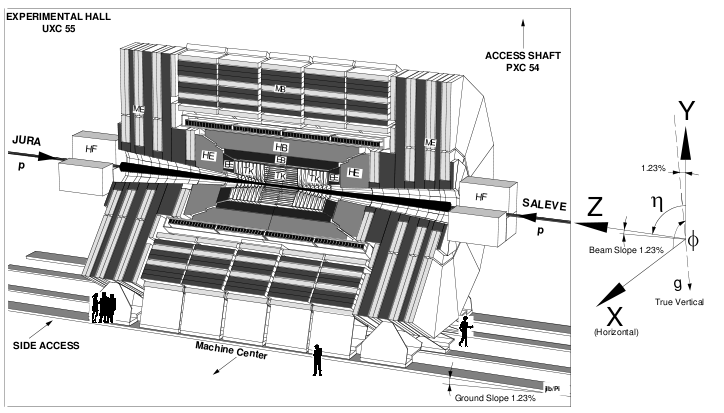
\includegraphics[width=1\textwidth]{figures/cmsDetectorAndCoordinateSystem.png}
	\caption{All CMS detector components and the coordinate system used to describe particle kinematics.}
	\label{fig:cmsAndCoordinateSystem}
\end{figure}


A pseudorapidity of 0 pointed along the $y$ axis, while a pseudorapidity of $\infty$ pointed along the $z$ axis.
An equivalent definition of pseudorapidity in terms of the particle energy E and longitudinal 
momentum $p_{z}$ in the massless particle limit was:

\begin{equation}
	\eta \equiv \frac{1}{2}\ln{\frac{E+p_{z}}{E-p_{z}}}
\end{equation}

Pseudorapidity was used to describe particle trajectories instead of the angle $\theta$ for several reasons.  Particles 
produced by pp interactions were often boosted along the $z$ axis, but the degree of boost was never well 
defined because the momenta of the interacting partons could never be measured.  This boost affected the 
trajectories of particles in $\theta$, but did not affect particle trajectories measured in $\eta$.  In 
addition, the particles that caused radiation damage in CMS sub-detector systems were produced at 
a rate that scaled linearly with $\eta$.  Thus, in discussions where radiation damage or particle 
isolation played a role, ideas could be more clearly articulated using $\eta$.

The main variables used to quantify particle energies were transverse energy 
$E_{T} \equiv E/\cosh{\eta}$ and transverse momentum $p_{T} \equiv |p|/\cosh{\eta}$, while the distance between 
a particle and another point in the $(\eta, \phi)$ space was measured as $\Delta R \equiv \sqrt{\eta^{2} + \phi^{2}}$.  
Transverse momentum, the component of momentum perpendicular to the proton beam axis, and transverse energy, the 
analogous form of energy, were used because both were insensitive to the unknown $z$ momenta of the interacting partons.  

\section{The Silicon Tracker}
\label{sec:siTrackerDescription}
Built from separate silicon pixel and silicon strip trackers, the silicon tracker detected charged particles  
and measured their momenta, and identified interaction vertices where charged particles were produced.  Closest 
to the beam axis was the pixel tracker, which used small silicon pixels to pinpoint pp interaction vertices 
with $\mu$m precision.  Surrounding the pixel tracker were larger silicon strip detectors that measured the 
momenta of charged particles with better resolution.  Charged particles produced within the tracker acceptance of $|\eta| < 2.5$ created 
e-h pairs in the silicon pixel and strip trackers, and measuring those pairs was the basis for all tracker 
measurements.

The pixel tracker was built from small rectangular pixel detectors organized in two 
structures based on $|\eta|$.  In the barrel region ($0 < |\eta| \lesssim 1.2$) where the rate of radiation damage was 
low, individual pixel detectors were assembled in three concentric cylindrical shells centered on the $z$ axis.  In 
the endcap region ($1.2 \lesssim |\eta| \leq 2.5$) where the rate of radiation damage was high, two layers of pixel detectors were 
installed in a turbine pattern as shown in Figure \ref{fig:pixelTracker} \cite{pixelCommissioning}.  These pixel 
layers provided 2 or 3 measurements for every track, and primarily were used to reconstruct interaction 
vertices.

\begin{figure}[ht]
	\centering
	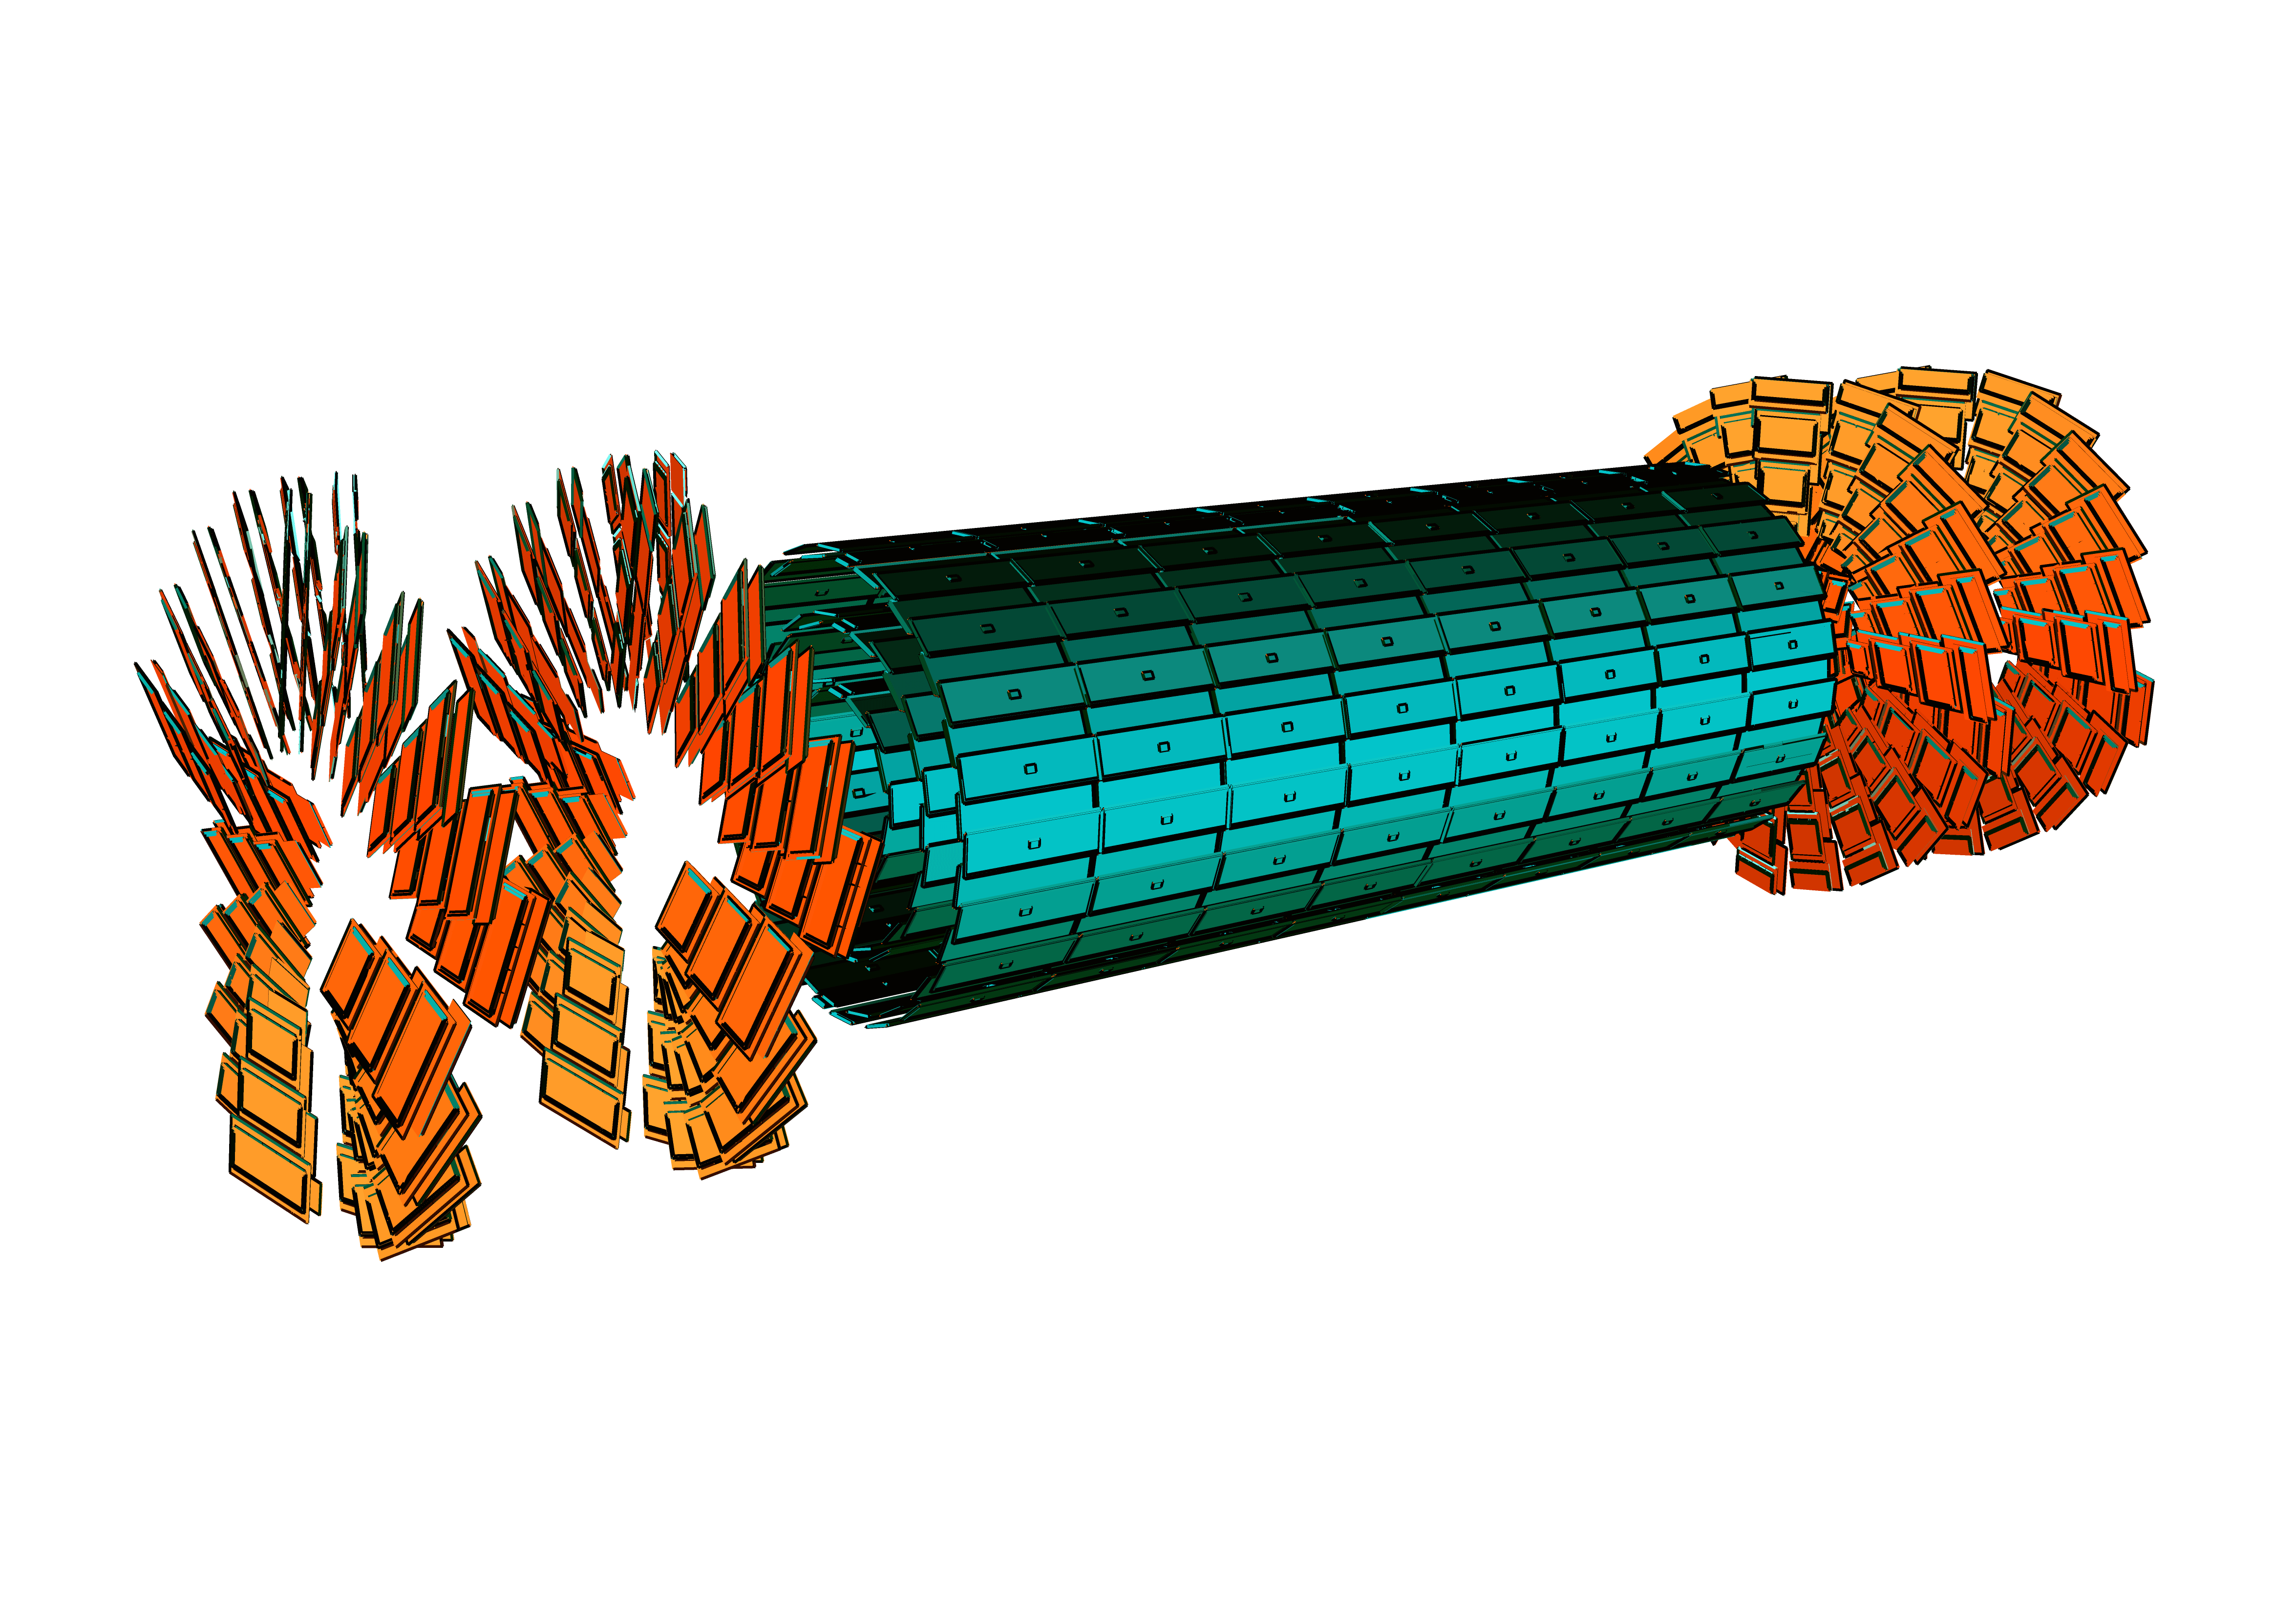
\includegraphics[width=0.8\textwidth]{figures/pixelDetectorSchematic.png}
	\caption{The barrel and endcap sections of the pixel tracker.}
	\label{fig:pixelTracker}
\end{figure}

Located outside the pixel tracker, the strip tracker was built from larger rectangular silicon detectors 
organized into four structures based on $|\eta|$, $|z|$ position and radius $r$ from the $z$ axis.  In the barrel region 
($0 < |\eta| \lesssim 1.2$), silicon strips were used to build 10 concentric cylindrical shells.  Similar to the pixel tracker, the strip tracker in 
the endcap region ($1.2 \lesssim |\eta| \leq 2.5$) used strip detectors arranged in disks.  As shown in Figure \ref{fig:stripTracker} 
\cite{cmsTDR}, silicon strips were used to build 12 endcap disk layers with some overlap in $|\eta|$ with the 
barrel strip detectors.  In the barrel and endcap regions several strip layers were built from pairs of closely spaced 
silicon strips that were slightly tilted relative to each other to measure track origins with better resolution.  The 
strip layers provided between 5 and 14 measurements for every track, and primarily were used to measure the momenta 
of charged particles.

\begin{figure}[ht]
	\centering
	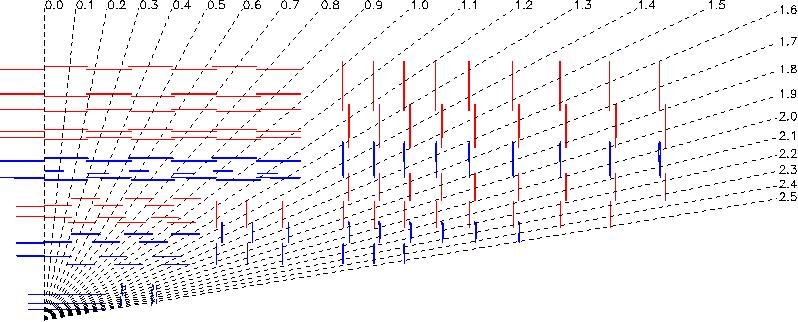
\includegraphics[width=0.8\textwidth]{figures/siliconStripAndPixelDetectorTwoDimView.png}
	\caption{The barrel and endcap sections of the silicon strip tracker for $\eta \geq 0.$ and one quadrant of $\phi$.  The pixel tracker is shown to scale in the bottom left corner.}
	\label{fig:stripTracker}
\end{figure}

Charged particles created e-h pairs in every pixel and strip detector they hit, and the total electron charge in such pairs was measured by readout 
modules attached to groups of pixels or strips\footnote{$\sim$16000 readout modules were connected to 66 million pixels, 
and $\sim$15400 readout modules were connected to 9.6 million strips.}.  
The granularity and multilayer structure of both detectors allowed the tracker to measure interaction vertex coordinates 
with $\lesssim 20\mu$m resolution along the $z$ axis, and with $\lesssim 10\mu$m resolution in the plane perpendicular to 
the $z$ axis, and measure the \pt of 100 GeV \pt muons with resolution better than 2\% in the barrel, and better than 
7\% in the endcap.

To measure interaction vertex positions and charged particle momenta with the quoted resolutions, the alignment and calibration 
of the tracker were measured before and during pp collisions in 2015.  Before collisions, cosmic ray muons were 
used to measure the tracker alignment and momentum response, and derive calibration factors that accounted for 
changes in either relative to expectations.  During collisions $Z \rightarrow \mu\mu$ events and cosmic ray muon events 
were used to monitor and recalibrate the tracker alignment and momentum response.


\section{The Electromagnetic Calorimeter}
\label{sec:ecalDescription}

Surrounding the silicon tracker was the electromagnetic calorimeter (ECAL), which detected photons, and distinguished
electrons and positrons ($e^{\pm}$) from other charged particles.  
The ECAL was an absorption calorimeter built from homogeneous, scintillating lead-tungstate (PbWO$_{4}$) crystals.  
In response to incident photons and $e^{\pm}$, the ECAL crystals emitted visible light in amounts proportional to 
the incident particle energy.  The ECAL measured the energies of photons and $e^{\pm}$ with $0 < |\eta| < 3.0$ by 
measuring the amount of visible light produced by PbWO$_{4}$ crystals.

The ECAL contained $\sim$76000 crystals divided into two $|\eta|$ regions based on the rate of radiation 
damage.  In the low $|\eta|$ barrel region ($0 < |\eta| < 1.479$) where the rate of radiation damage was low, 61200 
crystals that were 26 radiation lengths\footnote{On average a relativistic $e^{\pm}$ loses 63\% of its initial energy after 
travelling through one radiation length of material.} long were arranged in a cylindrical shell.  The front face of 
each crystal measured $\sim$22 $\times$ 22 \mm, and resided $\sim$19 \cm away from the outer most silicon tracker layer.  
In the endcap region ($1.479 < |\eta| < 3.0$) where the rate of radiation damage was high, 14648 crystals (half in each 
endcap) 25 radiation lengths long were installed in a disk.  The front face of endcap crystals measured $\sim$29 
$\times$ 29 \mm, and sat behind $\sim$2 radiation lengths of lead and silicon that constituted the preshower detector.  
The preshower mitigated radiation damage in endcap crystals, and improved the spatial resolution with 
which electromagnetic showers were studied in the endcap.  A partial view of the ECAL barrel, endcap and 
preshower detectors is shown in Figure \ref{fig:ecalEBEEandES} \cite{ecalTDR}.

\begin{figure}[ht]
	\centering
	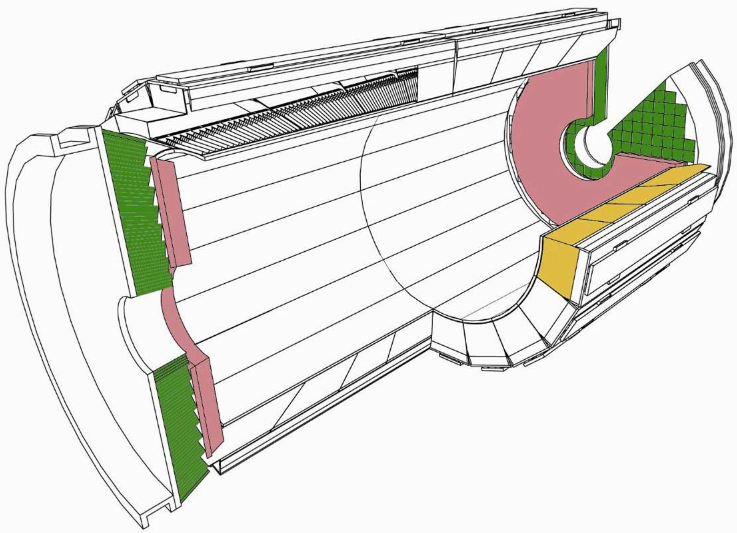
\includegraphics[width=0.8\textwidth]{figures/ecalBarrelEndcapAndPreshower.png}
	\caption{The ECAL barrel, endcap and preshower detectors.}
	\label{fig:ecalEBEEandES}
\end{figure}


Photons and $e^{\pm}$ that impinged on the ECAL interacted with lead-tungstate nuclei.  Incident photons 
converted into $e^{+}e^{-}$ pairs, and any energetic $e^{\pm}$ interacted with PbWO$_{4}$ nuclei through 
bremsstrahlung and produced gamma rays.  Gamma rays with sufficient energy converted into $e^{+}e^{-}$ pairs, 
and bremsstrahlung followed by pair conversion continued until more than 99.99\% of the initial photon or 
$e^{\pm}$ energy was lost.  For an incident photon or $e^{\pm}$ that did not interact with the silicon 
tracker, the resulting shower of low energy $e^{\pm}$ was usually fully contained in a 3 $\times$ 3 crystal 
grid centered on the most energetic crystal.

Showers of low energy $e^{\pm}$s interacted with lead-tungstate atoms and quickly produced distinguishable 
signals indicative of incident photon and $e^{\pm}$ energies.  Coulomb interactions between shower $e^{\pm}$s 
and bound state electrons in PbWO$_{4}$ atoms excited bound electrons to meta-stable states, and in 
$\lesssim$20 \ns more than 80\% of bound electrons returned to their ground states by emitting scintillation 
photons in the visible light regime.  The total energy of 
scintillation photons was measured by photodetectors to determine the incident photon or $e^{\pm}$ energy.  
The scintillating PbWO$_{4}$ and photodetectors enabled the ECAL to measure the energy of a 100 GeV photon or 
$e^{\pm}$ with resolution better than 1\% in the barrel region, and measure the energy of any incident photon or $e^{\pm}$ with 
resolution \cite{eGammaMonitCalib2011}:

\begin{equation}
	\frac{\sigma_{E}}{E} = \frac{2.8\%}{\sqrt{E/(1 GeV)}} \oplus \frac{0.151 GeV}{E} \oplus 0.3\%
\end{equation}

To measure photon and $e^{\pm}$ energies with the quoted resolution, the ECAL crystals were monitored and calibrated 
during data taking using several techniques.  Two to three times every hour each ECAL crystal was illuminated 
with light from one blue laser and one green laser to monitor the crystal transparency.  Every week laser data 
was used to calculate the average change in each crystal's transparency relative to the prior week, and this change 
was corrected by applying correction factors to the crystals.  Electrons and photons from $\eta \rightarrow \gamma\gamm$, 
$W \rightarrow e\nu$, and $Z \rightarrow e^{+}e^{-}$ were used to validate the weekly corrections derived from laser data.

To compliment weekly laser transparency corrections, $\sim$quarterly corrections were applied to ECAL crystals 
to calibrate their responses in terms of reconstructed particle energy.  Relative corrections were calculated from 
the weighted average relative correction determined using several methods described elsewhere \cite{eGammaMonitCalib2011}.  
The relative corrections normalized the responses of all crystals to the same value, then absolute scale corrections 
were applied.  The absolute correction for each crystal was derived using $e^{\pm}$ from $Z \rightarrow e^{+}e^{-}$, 
and ensured the average dilepton mass measured by each crystal in $Z \rightarrow e^{+}e^{-}$ events was equal to the 
true $Z$ boson mass.


\section{The Hadronic Calorimeter}
\label{sec:hcalDescription}
Surrounding the ECAL was the hadronic calorimeter (HCAL), which detected charged and neutral hadrons.  The 
HCAL was a sampling calorimeter built from alternating layers of thin scintillating plastic tiles and thick 
metal absorber plates.  Hadrons impinging on the HCAL interacted with the metal absorbers and produced amounts 
of visible light in the scintillating tiles proportional to their incident energies.  The HCAL 
measured the energies of hadrons with $0 < |\eta| < 3.0$ by measuring the amount of visible light produced 
by the scintillating tiles.

The HCAL consisted of 17 scintillating tile layers separated by 17 metal absorber layers.  Similar to the ECAL, the 
HCAL was divided into two $|\eta|$ regions based on the rate of radiation damage.  In the low $|\eta|$ barrel 
region ($0 < |\eta| < 1.4$), scintillating tiles and metal plates were organized into 2304 towers, and each 
covered the same area as a 5 $\times$ 5 grid of 
ECAL barrel crystals.  In the high $|\eta|$ ($1.3 < |\eta| < 3.0$) endcap region, scintillating 
tiles and absorber plates were assembled into 2304 towers (1152 per endcap), and each tower covered the same area 
as a 5 $\times$ 5 grid of ECAL endcap crystals.

Hadrons that impinged on the HCAL interacted with nuclei in metal absorber layers.  Diffractive and fully 
inelastic collisions between incident hadrons and absorber nuclei produced showers of lower 
energy hadrons that traveled into the nearest scintillating tile layers.  Incident hadrons with more energy yielded 
more particles in the shower.  Interactions between low energy hadrons and plastic molecules excited the molecules to 
higher energy states, and most molecules quickly de-excited and allowed scintillator molecules to produce scintillation 
light in $\lesssim$10 \ns.  This light was measured by photodetectors, and determined the energy of hadrons 
that impinged on the HCAL.  After calibrations the HCAL measured the energy of hadrons with the following resolution:

\begin{equation}
	\frac{\sigma_{E}}{E} = \frac{84.7\%}{\sqrt{E/(1 GeV)}} \oplus 7.4\%
\end{equation}

To maintain the energy resolution of the HCAL, the amount of light measured from towers of scintillating tiles 
was monitored and calibrated before and during 2015 collisions.  Before collisions, a radioactive source 
with known radioactivity was lowered into the HCAL, and the amount of scintillation light produced by each tile 
in response to the source was used to derive calibration constants.  Once collisions began, a laser system 
was used to monitor the efficiency of light transmission from scintillator tiles to the photodetectors.  
From laser transparency data, relative calibration constants were 
derived that normalized the response of all towers to hadronic activity to the same value.  The absolute 
calibration was determined by selecting events in which a jet recoiled off a photon, or a jet recoiled off a Z boson that 
decayed to a $e^{\pm}e^{\mp}$ or $\mu^{\pm}\mu^{\mp}$ pair.  In such events, the absolute hadronic energy 
scale was calibrated relative to the electromagnetic energy scale derived from $Z \rightarrow e^{\pm}e^{\mp}$ 
events.  Furthermore, the precision of the absolute hadronic energy scale calibration was improved using 
dijet resonances like $W/Z \rightarrow jj$.

\section{The Muon Detectors}
\label{sec:muonDetectorsDescription}
Outside the magnet were gas ionization chambers used to detect muons.  Muons that traversed the chambers 
ionized charge along their trajectories, and the ionized charges drifted through the gas to anodes and 
cathodes.  The muon detectors measured the momenta of muons with $0 < |\eta| < 2.4$ by measuring the amount of 
charge collected on the anodes and cathodes.

Like the calorimeters, the muon detectors were separated into barrel and endcap sections.  Shown in Figure \ref{fig:muonBarrelAndEndcapDetectors}, in the barrel 
region ($0 < |\eta| < 1.2$) where the magnetic field strength, muon rate and background rate were low, drift 
tubes (DTs) and resistive plate chambers (RPCs) were used to measure the positions and 
and momenta of muons, and determine the collision event that produced them based on time information.  In the endcap 
region ($1.2 < |\eta| < 2.4$) where particle fluxes and magnetic field strengths were higher, RPCs and cathode 
strip chambers (CSCs) were used to measure the same quantities.

\begin{figure}[ht]
	\centering
	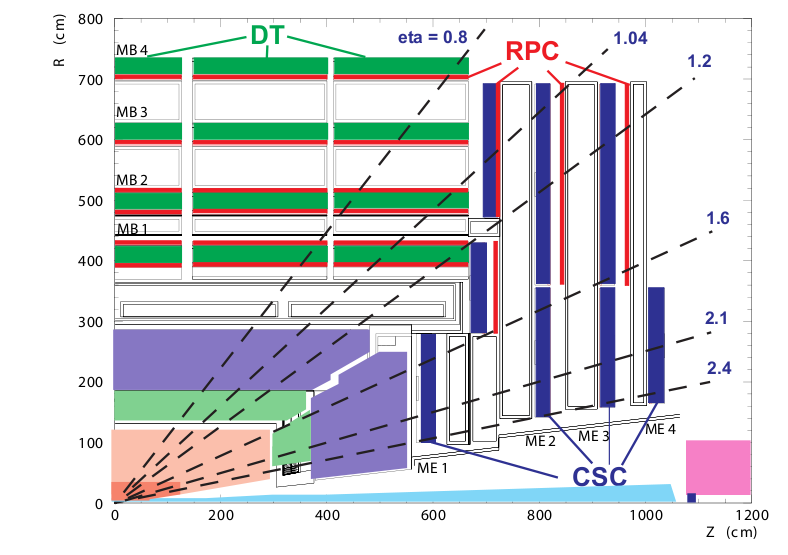
\includegraphics[width=0.8\textwidth]{figures/muonDetectorLayout.png}
	\caption{The barrel and endcap sections of the muon detectors for $\eta \geq 0.$ and one quadrant of $\phi$.  Shown 
		between the muon detectors and the interaction point are the magnet solenoid and return yoke, the HCAL, the ECAL, 
		and the silicon tracker.}
	\label{fig:muonBarrelAndEndcapDetectors}
\end{figure}


The DTs were organized into 5 wheels, each with 4 radial layers or 'stations', and 12 $\phi$ segments per 
station covering 30 degrees in $\phi$.  Each DT chamber contained several planes of drift tubes to measure 
muon trajectories in $z$, and r-$\phi$.  These planes enabled each station of DTs to measure muon trajectories 
with resolution better than 100 $\mu$m in $z$ and $r$, and $\sim$1 \mrad in $\phi$.  The DTs were separated 
from the interaction point where muons were produced by 13 \ns or more\footnote{assuming muons traveled at the speed 
of light.}, so the collision event that produced any muon was identified by RPC detectors.  By measuring 
the muon arrival time with $\sim$1 \ns resolution, the RPCs uniquely identified the collision event that 
produced a muon.

Muons in the endcap region were detected by CSCs divided amongst four disks that faced the barrel region.  
The disks were segmented into several radial layers (rings of different radii), as shown in Figure \ref{fig:muonBarrelAndEndcapDetectors}, 
to improve the resolution that muon positions and momenta were measured.  Each station contained 18 or 36 
chambers, each with multiple measurement planes, which enabled muon trajectories to be measured with resolution 
better than 200 $\mu$m in position, and $\sim$10 \mrad in $\phi$.  Similar to the barrel region DTs, the large distance between the interaction 
point and endcap CSCs meant that muons emitted into the endcap took 13 \ns or longer to reach the first CSC 
disk closest to the interaction point.  To identify the collision event that produced a muon, RPCs were used 
to detect muon arrival times with $\sim$1 \ns resolution.

The muon detectors complimented measurements made by the tracker, and improved the resolution of muon 
momentum measurements for high $\pt$ muons relative to tracker only performance.  The 
strength of the magnetic field enabled the tracker to measure muon momenta in the $\pt <$ 
200 GeV phase space with 3 or more times better resolution than the muon detectors.  As muon $\pt$ increased 
above 200 GeV, muon trajectories approached straight line paths, and thus the the tracker momentum resolution degraded.  
Combining tracker and muon detector information for high $\pt$ muons improved the resolution with which a 
$\pt = 1$ TeV muon was measured in the central barrel region by $\sim$200\% relative to the momentum 
measurement made by the tracker alone.

\section{The Trigger System}
\label{sec:triggerDescription}
In 2015 the rate of pp collision events delivered by the LHC was several orders of magnitude greater than the 
rate that CMS could save collision events to permanent storage.  The LHC collided two proton bunches 
at a rate of 40 MHz, and in nearly every collision $\gtrsim$1 GeV of energy was detected in CMS.  Due to the large cross 
section of QCD multijet processes and leptonically decaying heavy quark processes, shown in Figure \ref{fig:smProductionXsxns}, CMS 
detected $\sim10^{6}$ collision events per second with energetic charged leptons or hadronic jets.  In 2015 
CMS was able to write $\sim10^{3}$ collision events per second to permanent storage, so a two level trigger 
system was used during collisions ('online') to select the best events for physics analyses and detector calibration.

\begin{figure}[h]
	\centering
	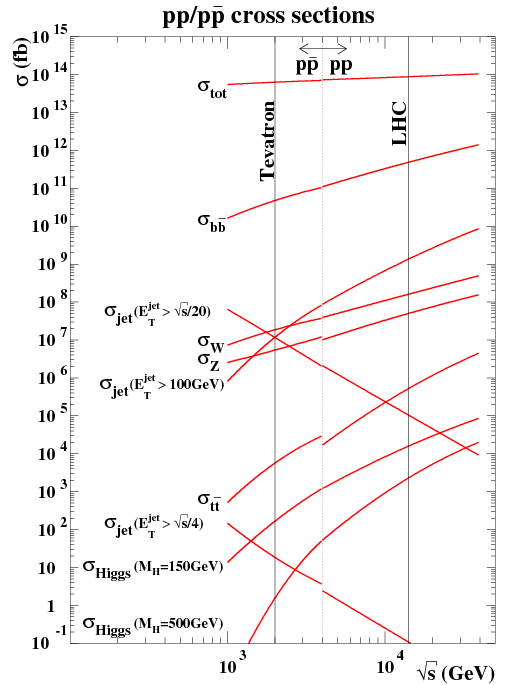
\includegraphics[width=0.6\textwidth]{figures/lhc_and_tevatron_cross_sections_2006.png}
	\caption{Production cross sections at the LHC and Tevatron as a function of center of mass energy.  Divide the cross section by $10^{5}$ to calculate 
	the approximate 2015 LHC production rate in events per second.}
	\label{fig:smProductionXsxns}
\end{figure}

By discarding collision events where no photons, charged leptons, hadronic jets, or neutrinos were 
detected, the Level-1 (L1) trigger system reduced the rate of collision events sent to the second 
level trigger system from 40 MHz to $\lesssim$ 80 kHz.  After every collision event, data from 
the ECAL, the HCAL and the muon detectors was used to build 'trigger 
primitive' objects that represented photons, muons and other particles.  In $\sim$1 $\mu$s these objects, 
distinguished by $E_{T}$ values and $(\eta, \phi)$ coordinates, were built and sent to the L1 logic system located 
$\sim$20 meters from CMS.  Implemented in programmable hardware like Field Programmable Gate Arrays, the L1 
logic system executed $\sim$200 algorithms in less than 1 $\mu$s that selected trigger primitive objects passing $E_{T}$ 
and $|\eta|$ selections.  The selection results were sent back to the detector, and the regions with one 
or more trigger primitive objects passing selections were processed by the second level trigger.

By selecting only the events needed for physics analyses and detector calibration, the second 
level, or High Level, trigger (HLT) reduced the rate of collision events written to permanent storage 
from $\lesssim$ 80 kHz to $\lesssim$ 1000 Hz.  The second level trigger began by transferring all data from the tracker, 
both calorimeters and the muon detectors to multi-core processors where the HLT was run\footnote{the same HLT software was run on every processor}.  
Then, the HLT ran a fast, simplified version of the full offline particle reconstruction software in small 
regions where L1 trigger algorithms fired.  Then, $\sim$400 HLT algorithms running in 
parallel applied selection cuts ($E_{T}$, $|\eta|$, $\frac{E_{HCAL}}{E_{ECAL}}$, etc) to locally reconstructed particles in search of 
energetic photons, charged leptons, hadronic jets, and neutrinos.  If the event passed at least one 
HLT algorithm, then the data from the entire detector was written to permanent storage.
Considering events selected by any HLT algorithm, during 2015 pp collisions the rate of data written to 
permanent storage was $\lesssim 0.5$ gigabytes per second.

